\def\mytitle{GATE ASSIGNMENT }
\def\myauthor{Vooribindi Chandini}
\def\mycontact{chandini.vooribindi@gmail.com}
\def\mymodule{IITH-Future Wireless Communication}

\documentclass[journal,12pt,twocolumn]{IEEEtran}
\usepackage{graphicx} 
\usepackage{enumitem}
\usepackage{tikz}
\usepackage{circuitikz}
\usepackage{karnaugh-map}
\usepackage{tabularx}
\title{\mytitle}
\author{\myauthor\\\mycontact\\IITH\hspace{0.3em}-\hspace{0.3em}\mymodule}
\begin{document}
\maketitle
\tableofcontents

\section{\textbf{Question}}
\begin{enumerate}
    \item  Which one of the following options is CORRECT for the given logic circuit?
\end{enumerate}
\vspace{1.0mm}
\begin{enumerate}[label=(\alph*)]
    \item P = 1, Q = 1; X = 0
    \item P = 1, Q = 0; X = 0
    \item P = 0, Q = 1; X = 0
    \item P = 0, Q = 0; X = 1
\end{enumerate}
    \section{\textbf{Answer}}
    $\rightarrow P'+ Q$\\
    Therefore, the Boolean function $F(X)=(P' + Q)$
   \section{\textbf{Logic Diagram}}
\begin{center}
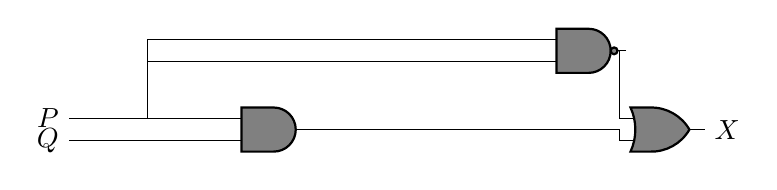
\begin{tikzpicture}
  \ctikzset{
    logic ports=ieee,
    logic ports/scale=0.5,
    logic ports/fill=gray}
      \node[and port](a) at (2,-2){};
        \node[ nand port](b) at (6,-1){};
                \node[or port](f) at (7,-2){};
                
          \draw(b.out)-|(f.in 1);
          \draw(a.out)-|(f.in 2);
          \draw(b.in 1)-| ++(-5,-1);
          \draw(b.in 2)-| ++(-5,0);
  \draw(a.in 1)-- ++(-2,0) node[left]{$P$};
  \draw(a.in 2)-- ++(-2,0) node[left]{$Q$};
  \draw(f.out)-- ++(0,0)node[right]{$X$};
  
\end{tikzpicture}
    
\begin{center}
Fig. 1 
\end{center}
       \end{center}
    %   \begin{center}
           \section{\textbf{Truth Table}}
\begin{tabularx}{0.45\textwidth}{
  | >{\centering\arraybackslash}X  
  %| >{\centering\arraybackslash}X 
  %| >{\centering\arraybackslash}X
 % | >{\centering\arraybackslash}X 
 % | >{\centering\arraybackslash}X 
  %| >{\centering\arraybackslash}X 
 % | >{\centering\arraybackslash}X 
  | >{\centering\arraybackslash}X 
  | >{\centering\arraybackslash}X 
  | >{\centering\arraybackslash}X 
  | >{\centering\arraybackslash}X |
  }
  \hline
  \textbf{$P$}&\textbf{$Q$}&\textbf{$P.Q$}&\textbf{$P'$}&\textbf{$X$}\\
  \hline
  0&0&0&1&1\\
  \hline
  0&1&0&1&1\\
  \hline
  1&0&0&0&0\\
  \hline
  1&1&1&0&1\\
  \hline
  
    \end{tabularx}
     \begin{center}
 Truth table for Boolean Function $X$
\end{center}
%\end{center}
    \section{\textbf{K-Map Implementation}}
    Using the boolean logic output $F$ can be expressed in terms of the inputs $X,Y,Z$ with the help of the following Kmap.
\\
    \begin{center}
      \resizebox{0.45\textwidth}{!}{%
      \begin{karnaugh-map}[2][2][1][$P$][$Q$]
            \maxterms{2}
            \minterms{0,1,3}
            \implicant{0}{1}{3}
            \implicant{1}{3}
            %\implicantedge{0}{0}{2}{2}
        \end{karnaugh-map}%
        }
    \end{center}
    \begin{center}
Fig. 2
\end{center}
\begin{center}
    \section{\textbf{Components}}
  \begin{tabularx}{0.45\textwidth} { 
  | >{\centering\arraybackslash}X 
  | >{\centering\arraybackslash}X 
  | >{\centering\arraybackslash}X
  | >{\centering\arraybackslash}X | }
\hline
 \textbf{Component}& \textbf{Values} & \textbf{Quantity}\\
\hline
Arduino & UNO & 1 \\  
\hline
LED & & 1 \\
\hline
Resistor& 220ohms & 1 \\
\hline
Jumper Wires& M-M & 5 \\ 
\hline
Breadboard &  & 1 \\
\hline
\end{tabularx}
\end{center}
\begin{center}
    \section{\textbf{Implementation}}
  \begin{tabularx}{0.46\textwidth} { 
  | >{\centering\arraybackslash}X 
  | >{\centering\arraybackslash}X 
  |>{\centering\arraybackslash}X  | }


\hline
\textbf{Arduino PIN} & \textbf{INPUT} & \textbf{OUTPUT} \\ 
\hline
\textbf 2 & P & \\
\hline
\textbf 3 & Q & \\
\hline
%\textbf 4 & Z & \\
%\hline
\textbf {13} & & X\\
\hline
\end{tabularx}
\end{center}
\begin{center}
    Connections
\end{center}

\textbf{Procedure}\\
1. Connect the circuit as per the above table.\\
2. Connect inputs to Vcc for logic 1, ground for logic 0.\\
3. Execute the circuit using the below code.\\
\\\begin{tabularx}{0.45\textwidth} { 
  | >{\centering\arraybackslash}X |
 % | >{\centering\arraybackslash}X |
 }
  \hline
https://github.com/Chandinivooribindi/gate2023\\
  \hline
\end{tabularx}\\
\\4. Change the values of P,Q in the code and verify the Truth Table.\\
\end{document}
